\let\negmedspace\undefined
\let\negthickspace\undefined
\documentclass[journal]{IEEEtran}
\usepackage[a5paper, margin=10mm, onecolumn]{geometry}
\usepackage{lmodern} % Ensure lmodern is loaded for pdflatex
\usepackage{tfrupee} % Include tfrupee package

\setlength{\headheight}{1cm} % Set the height of the header box
\setlength{\headsep}{0mm}     % Set the distance between the header box and the top of the text

\usepackage{gvv-book}
\usepackage{gvv}
\usepackage{cite}
\usepackage{amsmath,amssymb,amsfonts,amsthm}
\usepackage{algorithmic}
\usepackage{graphicx}
\graphicspath{{./figs/}}
\usepackage{textcomp}
\usepackage{xcolor}
\usepackage{txfonts}
\usepackage{listings}
\usepackage{enumitem}
\usepackage{mathtools}
\usepackage{gensymb}
\usepackage{comment}
\usepackage[breaklinks=true]{hyperref}
\usepackage{tkz-euclide} 
\usepackage{listings}
\usepackage{gvv}                                        
\def\inputGnumericTable{}                                 
\usepackage[latin1]{inputenc}                                
\usepackage{color}                                            
\usepackage{array}                                            
\usepackage{longtable}                                       
\usepackage{calc}                                             
\usepackage{multirow}                                         
\usepackage{hhline}                                           
\usepackage{ifthen}                                           
\usepackage{lscape}
\usepackage{circuitikz}
\tikzstyle{block} = [rectangle, draw, fill=blue!20, 
text width=4em, text centered, rounded corners, minimum height=3em]
\tikzstyle{sum} = [draw, fill=blue!10, circle, minimum size=1cm, node distance=1.5cm]
\tikzstyle{input} = [coordinate]
\tikzstyle{output} = [coordinate]


\begin{document}
	
	\bibliographystyle{IEEEtran}
	\vspace{3cm}
	
	\title{1.9.30}
	\author{EE25BTECH11042 - Nipun Dasari}
	\maketitle
	% \newpage
	% \bigskip
	{\let\newpage\relax\maketitle}
	
	\renewcommand{\thefigure}{\theenumi}
	\renewcommand{\thetable}{\theenumi}
	\setlength{\intextsep}{10pt} % Space between text and floats
	
	
	\numberwithin{equation}{enumi}
	\numberwithin{figure}{enumi}
	\renewcommand{\thetable}{\theenumi}
	
	\textbf{Question}:\\
	If the distances of $\vec{P} = \brak{x, y}$ from $\vec{A} = \brak{5, 1}$ and $\vec{B} = \brak{−1, 5}$are equal, then prove
	that $3x = 2y$.
	
	\solution \\
	Consider the matrices A, B and P as follows:
	\begin{align*}
		\vec{A} = \myvec{5 \\ 1}, \vec{B} = \myvec{-1 \\ 5}, \vec{P}= \myvec{x \\ y}
	\end{align*}
	The condition for distances from $\vec{B}$ to $\vec{P}$ and $\vec{A}$ to $\vec{P}$ to be equal is
	\begin{align*}
		\norm{\vec{P}-\vec{A}} = \norm{\vec{P}-\vec{B}} \equiv \norm{\vec{P}-\vec{A}}^2 = \norm{\vec{P}-\vec{B}}^2
	\end{align*}
	Using inner products:
	\begin{align*}
		\brak{\vec{P}-\vec{A}}^{T}\brak{\vec{P}-\vec{A}} = \brak{\vec{P}-\vec{B}}^{T}\brak{\vec{P}-\vec{B}}
	\end{align*}
	Expanding on both sides:
	\begin{align*}
		\vec{P}\vec{P}^{T} - 2\vec{A}^{T}\vec{P} + \vec{A}^{T}\vec{A} = \vec{P}\vec{P}^{T} - 2\vec{B}^{T}\vec{P} + \vec{B}^{T}\vec{B}
	\end{align*}
	On simplification:
	\begin{align*}
		\brak{-2\vec{A}^{T} + 2\vec{B}^{T}}\vec{P} = \vec{B}^{T}\vec{B} - \vec{A}^{T}\vec{A}
	\end{align*} 
	LHS constant matrix:
	\begin{align*}
	2\brak{\vec{B}-\vec{A}}^{T} = 2\myvec{-1-5 \\ 5-1} = \myvec{-12 & 8}	
	\end{align*}
	RHS constant matrix:
	\begin{align*}
		\vec{B}^{T}\vec{B} - \vec{A}^{T}\vec{A} = \brak{\brak{-1}^2 + 5^2} - \brak{1^2 + 5^2} = 0
	\end{align*}
	From the above:
	\begin{align*}
		\myvec{-12 & 8}\myvec{x \\ y} = 0 \implies -12x + 8y = 0 \implies 3x = 2y
	\end{align*}
	From the plot we can infer that the locus is perpendicular bisector of the line joining the 2 vectors 
	\begin{figure}[H]
		\centering
		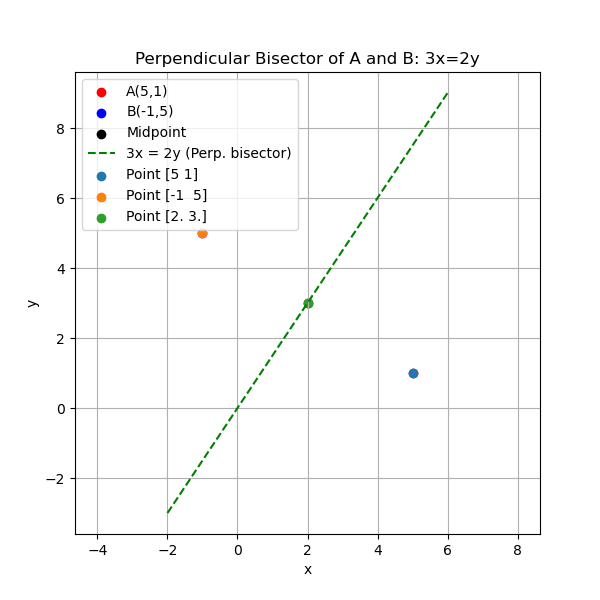
\includegraphics[width = 0.8\columnwidth]{fig.png}
		\caption*{}
		\label{fig}
	\end{figure}
\end{document}